\documentclass[a4paper,11pt,fleqn]{article}%fleqn pour aligner les equations à gauche
\usepackage{../../Styles/Exercice}
\usepackage{xfp}


\newcommand{\chnum}{Chapitre 3}
\newcommand{\chtitle}{Cinétique chimique}
\newcommand{\dtype}{Exercices corrigés}

\begin{document}
\maketitle
\begin{multicols}{2}
\section{Identifier un facteur cinétique}
Les mélanges ci-dessous sont réalisés à partir d'une solution de concentration en quantité d'iodure de potassium $C_1$ = \num{0,20} \unit{\mole\per\liter} et d'une solution de concentration en quantité d'acide sulfurique $c_2$ = \num{0,50} \unit{\mole\per\liter}.

\begin{table}[h!]
    \centering
    \begin{tabular}{|>{\centering}m{3cm}|>{\centering}m{3cm}|>{\centering}m{3cm}|>{\centering\arraybackslash}m{3cm}|}
    \hline Mélange & n°1 & n°2 & n°3\\
    \hline $V_1$ (en \unit{\milli\liter}) & 10 & 20 & 30\\
    \hline $V_2$ (en \unit{\milli\liter}) & 10 & 10 & 10\\
    \hline $V_3$ (en \unit{\milli\liter}) & 30 & 20 & 10\\
    \hline
    \end{tabular}
    \label{tab:my_label}
\end{table}

$V_1$ désigne le volume de solution d'iodure de potassium, $V_2$ le volume de solution d'acide sulfurique et $V_3$ le volume d'eau ajoutée.\\
Au même instant, dans chaque bécher est versé une solution de concentration en quantité de péroxyde d'hydrogène $c_4$ = \num{10} \unit{\milli\mole\per\liter} et de volume $V_4$ = \num{50} \unit{\milli\liter}. Au bout de deux minutes, la coloration jaune (caractéristique de la présence de diiode) est de plus en plus foncée du bécher 1 au bécher 3.\\
L'équation de la réaction qui modélise la transformation est :
\begin{eqnarray}
\ce{H2O2(aq) + 2H+(aq) + 2I-(aq) -> 2H2O(l) + I2(aq)} \nonumber
\end{eqnarray}
\begin{enumerate}
    \item Expliquer les colorations de plus en plus foncées observées au même instant du bécher 1 au bécher 3.\\
    \textcolor{blue}{Les colorations foncées viennent de l'apparition de diiode dans chaque bécher à des vitesses différentes.}
    \item Montrer que, quel que soit le mélange, le réactif limitant est le peroxyde d'hydrogène \ce{H2O2}.\\
    \textcolor{blue}{On constate que, quelle que soit le mélange les quantités de peroxyde d'hydrogène est la même : $n_{\ce{H2O2}} = c_4 \times V_4 = \num{10e-3} \times \num{50e-3}$ = \num{5,0e-4} \unit{\mole}. \textcolor{olive}{$x_{max}$ = \num{5,0e-4} \unit{\mole}}\\
    de même la quantité d'acide sulfurique est la même dans chaque expérience :\\
    $n_{\ce{H+}} = c_2 \times v_2 = \num{0,50} \times \num{10e-3}$ = \num{5,0e-3} \unit{\mole}. \textcolor{orange}{$x_{max}$ = \num{2,5e-3} \unit{\mole}}\\
    Il ne reste que la quantité d'ions iodure à déterminer : }\\
    \begin{tabular}{|c|c|c|}
    \hline Mélange & $n_{\ce{I-}}$ & $x_{max}$\\
    \hline 1 & \num{2e-3} & \num{1e-3}\\
    \hline 2 & \num{4e-3} & \num{2e-3}\\
    \hline 3 & \num{6e-3} & \num{3e-3}\\
    \hline
    \end{tabular}\\
    \textcolor{blue}{On constate que la valeur de $x_{max}$ la plus faible est toujours celle du peroxyde d'hydrogène, il sera donc le réactif limitant dans chacun des cas.}
    \item En déduire la quantité de matière, puis la concentration en quantité de diiode finales dans chaque mélange.\\
    \textcolor{blue}{Puisque le réactif limitant est toujours le péroxyde d'hydrogène, on aura toujours $n_{\ce{I2}} = x_{max} = \SI{5,2E-4}{mol}$ }
    \item Déterminer alors s'il subsiste une différence d'intensité de coloration d'un bécher à un autre.\\
    \textcolor{blue}{Les trois béchers auront au final la même concentration en diiode et donc la même teinte. Cependant on constate que la concentration en iodure est croissante du bécher 1 au 3. La concentration en réactif étant un facteur cinétique favorisant la vitesse de réaction, il parait donc normal que les béchers les plus concentrés affichent plus rapidement une teinte foncée que les béchers ayant une concentration plus faible.}
\end{enumerate}

\section{Stabilité de l'eau de Javel}
L'eau de Javel (solution d'hypochlorite de sodium (\ce{Na+(aq)},\ce{Cl-(aq)}), solution désinfectante, doit être conservée au frais, à l'abri de l'air et de la lumière. En effet, l'ion hypochlorite se transforme selon la réaction d'équation :
\begin{eqnarray}
    \ce{2ClO-(aq) -> 2Cl-(aq) + O2(g)}\nonumber
\end{eqnarray}
La concentration en quantité d'ion hypochlorite d'un flacon d'eau de Javel est donnée ci-dessous à différentes dates pour deux solutions $S_1$ et $S_2$ différentes (à la température de \num{20} \unit{\celsius}).
\\
    \begin{tabular}{|c|c|c|c|c|c|c|}
    \hline t (en jours) & 0 & 50 & 100 & 150 & 200 \\
    \hline $c_1$ (en \unit{\mole\per\liter}) & 2,00 & 1,65 & 1,36 & 1,12 & 0,92\\
    \hline $c_2$ (en \unit{\mole\per\liter}) & 1,60 & 1,32 & 1,09 & 0,89 & 0,74\\
    \hline
    \end{tabular}\\
\noindent
    \begin{tabular}{|c|c|c|c|c|c|}
    \hline t (en jours) & 250 & 300 & 350 & 400\\
    \hline $c_1$ (en \unit{\mole\per\liter}) & 0,76 & 0,63 & 0,52 & 0,42\\
    \hline $c_2$ (en \unit{\mole\per\liter}) & 0,61 & 0,50 & 0,41 & 0,34\\
    \hline
    \end{tabular}

\begin{enumerate}
    \item Proposer une argumentation permettant de déterminer s'il est préférable de conserver des solutions d'eau de Javel concentrées ou diluées.\\
    \textcolor{blue}{Une concentration plus élevée d'eau de Javel permet de garder une concentration plus importante sur une durée plus longue dans le temps. L'efficacité de la solution étant directement liée à sa concentration, il vaudrait mieux la conserver sous forme concentrée pour garder une activité sur le plus long terme.}
    \item Proposer une expérience permettant de vérifier la recommandation faite par le fabricant de conserver l'eau de Javel au frais.\\
    \textcolor{blue}{Il serait intéressant de partir de deux solution de même concentration en ions hypochlorite. Une première solution est placée au frais au réfrigérateur alors que la deuxième est laissée à température ambiante. Des prélèvements sont réalisés à intervalles de temps réguliers sur 400 jours de manière à suivre la concentration en ions hypochlorite au cours du temps.}
    \item Dessiner l'allure des courbes attendues lors de cette expérience.\\
    \textcolor{blue}{On remarque que la solution gardée au réfrigérateur a une vitesse de réaction moins importante (en bleu) par rapport à la solution gardée à température ambiante (en rouge).}
\end{enumerate}
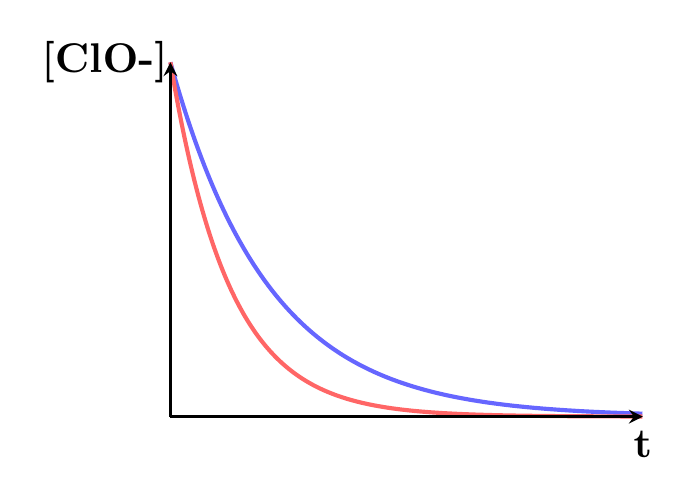
\begin{tikzpicture}[scale = 1.5, transform shape]
    \draw [domain=0:4,samples = 300,blue!60,line width = 1.5pt] plot (\x,{3*exp(-1.2*\x)});
    \draw [domain=0:4,samples = 300,red!60,line width = 1.5pt] plot (\x,{3*exp(-2*\x)});
    \draw[-stealth,very thick] (0.0,0) to (0,3);
    \draw[-stealth,very thick] (0.0,0) to (4,0);
%\draw[dashed] (0.5,0) --(0.5,.7);
    \draw (4,0) node[below]{\textbf{t}};
%\draw (.5,0) node{$|$} node[below]{\Large $t_1$};
    \draw (0.1,3) node[left]{$\textbf{[\ce{ClO-}]}$};
%\draw (2,2) node[right]{\Large $v_{disp}(R)_t = \dfrac{-\Delta [R]}{\Delta t}$};
\end{tikzpicture}

\section{Transformer des gaz}
Le pentoxyde de diazote de formule \ce{N2O5} permet de réaliser des réactions chimiques de nitration pour l'obtention d'espèces explosives, comme le TNT. Le suivi temporel de sa décomposition à \num{343} \unit{\kelvin} est effectué dans une enceinte fermée de volume constant par mesure de la pression $P$ au cours du temps. Cette décomposition est modélisée par la réaction d'équation :
\begin{eqnarray}
    \ce{2N2O5(g) -> 4NO2(g) + O2(g)}\nonumber
\end{eqnarray}
Les résultats obtenus sont donnés ci-dessous.
\\
\begin{tabular}{|c|c|c|c|c|c|c|c|c|c|c|}
    \hline $t$ (en min) & 0 & 10 & 20 & 30 & 40 & 50 & 60 & 70 & 80 & 100\\
    \hline $P$ (en bar) & 0,354 & 0,490 & 0,593 & 0,670 & 0,726 & 0,764 & 0,794 & 0,820 & 0,837 & 0,858\\
    \hline
\end{tabular}
\textbf{Données :}\\
\begin{itemize}
    \item La concentration en quantité de matière d'une espèce gazeuse est définie par : $[\ce{N2O5}] = \dfrac{n_{\ce{N2O5}}}{V}$ où $V$ est le volume du gaz.
    \item Une analyse permet d'établir : $[\ce{N2O5}] = \dfrac{5P_0-2P}{3RT}$ avec $P_0$ la pression initiale en \unit{\pascal} (1 bar = \num{1e5} \unit{\pascal}), $R$ = \num{8,31} \unit{\joule\per\mole\per\kelvin}, $T$ la température  en kelvin et [\ce{N2O5}] en \unit{\mole\per\meter\cubed}.
\end{itemize}
\begin{enumerate}
    \item Calculer la vitesse volumique de consommation de \ce{N2O5} à $t$ = 0.\\
    \textcolor{blue}{Pour avoir accès à la vitesse volumique, il faut calculer les valeurs de concentration [\ce{N2O5}] pour chaque temps donnés. \emph{Attention : la pression doit être convertie en Pascal.}}\\
\end{enumerate}

\begin{tabular}{|c|c|} \hline
    t (min) & $[\ce{C2O5}]$ (en \unit{\mole\per\liter})\\
    \hline
    0 & 12.4\\
    10 & 9.24\\
    20 & 6.83\\
    30 & 5.03\\
    40 & 3.72\\
    50 & 2.83\\
    60 & 2.13\\
    70 & 1.52\\
    80 & 1.12\\
    100 & 0.632\\
    \hline
\end{tabular}\\
\textcolor{blue}{Pour trouver la vitesse à l'origine il faut tracer la tangente à l'origine puis en déterminer la pente :}
\begin{center}
\begin{tikzpicture}[scale = .7, transform shape]
    \draw[-Stealth] (0,0) to (12,0);
    \draw[-Stealth] (0,0) to (0,11);
    \foreach \t in {0,1,2,3,4,5,6,7,8,9,10} {
        \pgfmathsetmacro\x{10*\t}
        \pgfmathsetmacro\c{12.42*exp{-0.298*\t}}
        \draw (\t,\c) node{\Large$\mathbf{\times}$};
        \draw (\t,-.1) -- (\t,.1);
        \draw (\t,-.2) node[below]{\pgfmathprintnumber[precision=1]{\x}};
    }
    \foreach \i in {0,2,...,12}{
        \draw (-.1,\i) -- (.1,\i);
        \draw (-.1,\i) node[left]{\pgfmathprintnumber[precision=1]{\i}};
    }
    \draw [domain=0:.8,color =blue, thick, dashed] plot (\x, {-12.42*\x + 12.42} );
    \draw (0,12.5) node[above]{$[\ce{C2O5}]$};
    \draw (11,0) node[above]{$t (min)$};
\end{tikzpicture}
\end{center}

\textcolor{blue}{On observe une tangente à l'origine qui a une pente d'une valeur absolue d'environ \SI{12,4}{\mole\per\liter\per\second} correspondant à la vitesse volumique de disparition de \ce{N2O5}}

\begin{enumerate}[resume]
    \item Vérifier que l'évolution de [\ce{N2O5}] suit une loi de vitesse d'ordre 1.
\end{enumerate}
\textcolor{blue}{Pour vérifier, à partir des données, l'ordre de la réaction il faut  étudier la fonction de décroissance exponentielle :
$$[\ce{C2O5}] =[\ce{C2O5}]_0 \cdot e^{-k\cdot t} $$
Il est possible de déterminer $k$ en transformant cette fonction pour l'isoler :
$$\dfrac{[\ce{C2O5}]}{[\ce{C2O5}]_0} = e^{-k\cdot t}$$
$$ln\left(\dfrac{[\ce{C2O5}]}{[\ce{C2O5}]_0}\right) = -k\cdot t$$
Cette relation montre que la si l'on trace $ln\left(\dfrac{[\ce{C2O5}]}{[\ce{C2O5}]_0}\right)$ en fonction du temps, pour une réaction suivant une loi de vitesse d'ordre 1, alors on obtiendra une droite de pente décroissante qui aura pour valeur absolue $k$ la constante de vitesse.}
\begin{center}
\begin{tikzpicture}[scale = .7, transform shape]
    \draw[-Stealth] (0,0) to (11,0);
    \draw[-Stealth] (0,0) to (0,-4);
    \foreach \t in {0,1,2,3,4,5,6,7,8,9,10} {
        \pgfmathsetmacro\c{-0.298*\t}
        \pgfmathsetmacro\x{10*\t}
        \draw (\t,\c) node{\Large$\mathbf{\times}$};
        \draw (\t,-.1) -- (\t,.1);
        \draw (\t,.1) node[above]{\pgfmathprintnumber[precision=1]{\x}};
    }
    \foreach \i in {0,-1,...,-3}{
        \draw (-.1,\i) -- (.1,\i);
        \draw (-.1,\i) node[left]{\pgfmathprintnumber[precision=1]{\i}};
    }
    \draw [domain=0:10,color =blue, thick, dashed] plot (\x, {-.298*\x} );
    \draw (9,-1) node{$y = -0.0298\cdot x$};
    \draw (0,-4) node[below]{$ln\left(\dfrac{[\ce{C2O5}]}{[\ce{C2O5}]_0}\right)$};
    \draw (11,.5) node[above]{$t (min)$};
\end{tikzpicture}
\end{center}


\section{Modéliser un nuage de points}
La décomposition de l'iodure d'hydrogène est modélisée par la réaction d'équation :
\begin{eqnarray}
    \ce{2HI(g) -> H2(g) + I2(g)}\nonumber
\end{eqnarray}
Le suivi temporel de cette transformation donne, à \num{580} \unit{\kelvin}, les résultats suivants :
\begin{center}
    \begin{tabular}{|>{\centering}m{.15\linewidth}|c|c|c|c|c|}
    \hline Temps (en s) & 0 & 1000 & 2000 & 3000 & 4000\\
    \hline [\ce{HI}] (en \unit{\mole\per\liter}) & 1,000 & 0,110 & 0,061 & 0,041 & 0,031\\
    \hline
    \end{tabular}
\end{center}

La concentration en quantité de matière d'une espèce gazeuse est définir comme celle d'une espèce dissoute : $[\ce{HI}] = \dfrac{n_{\ce{HI}}}{V}$ où $V$ est le volume du gaz et $[\ce{HI}]_0 = [\ce{HI}](0)$.
\begin{enumerate}
    \item Calculer, pour chaque date ci-dessus, $\ln{\dfrac{[\ce{HI}](t)}{[\ce{HI}]}}$.
\end{enumerate}
\textcolor{blue}{
    \begin{center}
    \begin{tabular}{|>{\centering}m{.15\linewidth}|c|c|c|c|c|}
    \hline Temps (en s) & 0 & 1000 & 2000 & 3000 & 4000\\
    \hline [\ce{HI}] (en \unit{\mole\per\liter}) & 1,000 & 0,110 & 0,061 & 0,041 & 0,031\\
    \hline \small $\ln{\dfrac{[\ce{HI}](t)}{[\ce{HI}]}}$ & 0,000 & -2,207 & -2.797 &-3,194& -3,474\\ \hline
    \end{tabular}
\end{center}}
\begin{enumerate}[resume]
    \item À l'aide d'une représentation graphique, déterminer si l'évolution de la concentration du iodure d'hydrogène suit une loi de vitesse d'ordre 1.
\end{enumerate}
\begin{center}
\begin{tikzpicture}[scale = 1.2, transform shape]
    \draw[-Stealth] (0,0) to (4.5,0);
    \draw[-Stealth] (0,0) to (0,-4.5);
    \draw (0,0) node{\Large$\mathbf{\times}$};
    \draw (1,-2.2) node{\Large$\mathbf{\times}$};
    \draw (2,-2.8) node{\Large$\mathbf{\times}$};
    \draw (3,-3.2) node{\Large$\mathbf{\times}$};
    \draw (4,-3.47) node{\Large$\mathbf{\times}$};
    \foreach \t in {0,1,2,3,4} {
        \pgfmathsetmacro\x{1000*\t}
        \draw (\t,-.1) -- (\t,.1);
        \draw (\t,.1) node[above]{\small \pgfmathprintnumber[precision=1]{\x}};
    }
    \foreach \i in {0,-1,...,-3}{
        \draw (-.1,\i) -- (.1,\i);
        \draw (-.1,\i) node[left]{\small \pgfmathprintnumber[precision=1]{\i}};
    }
    \draw (-.5,-4) node[left]{$ln\left(\dfrac{[\ce{HI}]}{[\ce{Hi}]_0}\right)$};
    \draw (4,.5) node[above]{$t (min)$};
\end{tikzpicture}
\end{center}

\textcolor{blue}{La représentation n'est pas une droite, il ne s'agit donc pas d'une réaction suivant une loi de vitesse d'ordre 1.}

\section{Purification de l'eau}
L'ozone \ce{O3} est utilisé dans le traitement de l'eau, pour la production d'eau potable et pour l'épuration des eaux industrielles. Lors du processus de purification, l'ozone est transformé en dioxygène, transformation modélisée par la réaction d'équation :
\begin{eqnarray}
    \ce{O3(aq) ->} \frac{3}{2} \ce{O2(aq)}\nonumber
\end{eqnarray}
L'évolution de la concentration en masse en ozone au cours du temps pour diverses concentrations en masse initiales en ozone dissous en présence de charbon actif est donnée ci-dessous (à la température de 20\unit{\celsius}).
\begin{center}
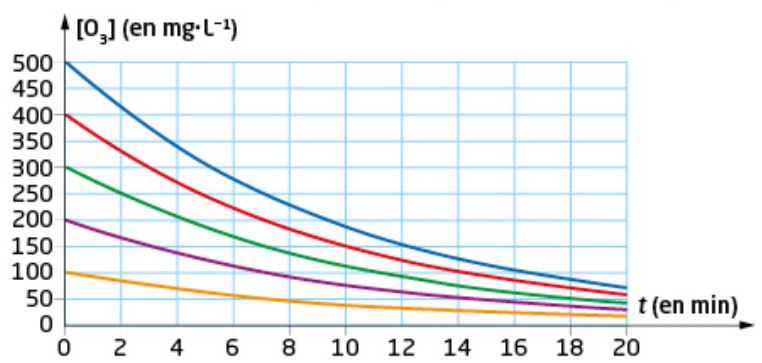
\includegraphics[width =\linewidth]{Ressources/TSPE_C10_Exercices_Fig1.png}
\end{center}
Par ailleurs, à la température de 20\unit{\celsius} en l'absence de charbon actif, le temps de demi-réaction vaut \num{13,1} \unit{\minute}.
\begin{enumerate}
    \item Déterminer, pour chaque concentration initiale, le temps de demi-réaction.
\end{enumerate}
\begin{tikzpicture}
    \node[anchor=south west,inner sep=0] (image) at (0,0) {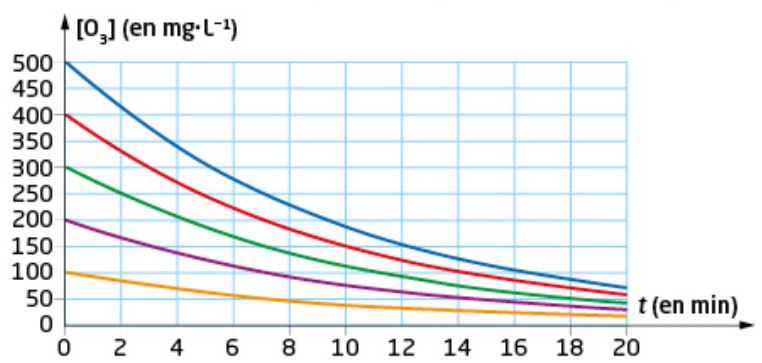
\includegraphics[width=\linewidth]{Ressources/TSPE_C10_Exercices_Fig1.png}};
    %\draw(0,0) grid(10,5);
    \draw[blue,thick,-stealth] (.8,2.1) to (3.3,2.1); \draw[blue,thick,-stealth] (3.3,2.1) to (3.3,.5);
    \draw[red,thick,-stealth] (.8,1.75) to (3.3,1.75); \draw[red,thick,-stealth] (3.3,1.75) to (3.3,.5);
    \draw[green!40!black,thick,-stealth] (.8,1.4) to (3.3,1.4); \draw[green!40!black,thick,-stealth] (3.3,1.4) to (3.3,.5);
    \draw[purple!40!black,thick,-stealth] (.8,1.1) to (3.3,1.1); \draw[purple!40!black,thick,-stealth] (3.3,1.1) to (3.3,.5);
    \draw[orange,thick,-stealth] (.8,.8) to (3.3,.8); \draw[orange,thick,-stealth] (3.3,.8) to (3.3,.5);
    \draw (3.3,0) node{$t_{1/2}$};
\end{tikzpicture}
\begin{enumerate}[resume]
    \item En déduire si l'évolution de la concentration en quantité d'ozone suit ou ne suit pas une loi d'ordre 1.
\end{enumerate}
\textcolor{blue}{On remarque que le temps de demi-réaction ne dépend pas de la concentration en réactif, ce qui indique qu'il s'agit d'une loi d'ordre 1.}
\begin{enumerate}[resume]
    \item Indiquer quel est le rôle du charbon actif.
\end{enumerate}
\textcolor{blue}{Dans ce cas le charbon actif est présent dans le milieu réactionnel mais il n'intervient pas dans l'équation de la réaction, il s'agit donc d'un catalyseur utilisé pour accélérer la réaction.}

%\newpage
\section{Un initiateur de polymère}
Le péroxyde de di\emph{tert}butyle, noté \textbf{A} est un amorceur de nombreuses réactions de polymérisation formant des matières plastiques.\\
Cette espèce chimique ne peut pas être utilisée à une température trop élevée car elle se décompose spontanément. Cette décomposition est modélisée par la réaction d'équation :
\begin{eqnarray}
    \small \ce{(H3C)3COOC(CH3)3(g) -> 2CH3COCH(g) + H3CCH3(g)}\nonumber
\end{eqnarray}
La mesure de la pression totale $P$ du mélange constitué initialement de \textbf{A} en quantité de matière $n_0$ = \num{10} \unit{\milli\mole}, dans une enceinte fermée de volume $V$ conduit aux résultats suivants :
\begin{center}
\begin{tabular}{|>{\centering}m{.2\linewidth}|c|c|c|c|c|c|}
    \hline Date $t$ (en \unit{\minute}) & 2,00 & 6,00 & 14,0 & 22,0 & 30,0 & 38,0 \\
    \hline Pression $P$ (en \unit{\kilo\pascal}) & 25,0 & 26,5 & 29,5 & 32,3 & 34,9 & 37,3\\
    \hline
\end{tabular}
\end{center}
Au bout d'une durée très longue, la mesure de la pression conduit à une valeur constante $P_{\infty}$ = \num{71,8} \unit{\kilo\pascal}.\\
\textbf{Données :}
\begin{itemize}
    \item La concentration en quantité d'une espèce gazeuse suit la même définition que celle d'une espèce dissoute : $[A] = \dfrac{n_A}{V}$ où $n_A$ est la quantité de matière de \textbf{A} et $V$ est le volume occupé par le gaz.
    \item Constante des gaz parfaits : $R$ = \num{8,31} \unit{\joule\per\mole\per\kelvin}.
\end{itemize}
\begin{enumerate}
    \item \textbf{Analyse des résultats expérimentaux}
    \begin{enumerate}
        \item À l'aide d'un tableau d'avancement et en admettant que la transformation est totale, montrer que $P_0 = \dfrac{P_{\infty}}{3}$.
        \item Exprimer à tout instant la concentration en quantité de \textbf{A}, notée $[A](t)$, en fonction de $P(t)$, $P_0$, $R$ et $T$.
        \item Tracer le nuage de points expérimental en plaçant le temps en abscisse et $\ln{\left(\dfrac{[A]}{[A]_0}\right)}$ en ordonnée. Modéliser la courbe passant au plus près de ce nuage de points par une équation adéquate. Noter l'équation obtenue.
    \end{enumerate}
    \item \textbf{Utilisation du modèle des réactions d'ordre 1}
    \begin{enumerate}
        \item Dans l'hypothèse où l'évolution de $[A](t)$ suit une loi de vitesse d'ordre 1 de constante de vitesse volumique $k$, établir l'équation différentielle liant $[A](t)$ à la valeur de sa dérivée par rapport au temps.
        \item Établir l'expression mathématique de $[A](t)$.
        \item Explique pourquoi les résultats expérimentaux sont en accord avec le modèle de la réaction d'ordre 1, puis donner la valeur numérique de $k$.
    \end{enumerate}
\end{enumerate}

1. (a) \textcolor{blue}{Tableau d'avancement :\\
\begin{center}
    \begin{tabular}{|c|c||c|c|}
    \hline Avancement & \multicolumn{3}{|c|}{\ce{A -> 2CH3COCH(g) + H3CCH3(g)}}\\
    \hline$x=0$& $n_i(A)$ & 0 & 0 \\
    \hline $x$ & $n_i(A)-x$ & $2x$ & $x$\\
    \hline $x_{max}$ & $n_i(A)-x_{max}$ & $2x_{max}$ & $x_{max}$\\
    \hline
    \end{tabular}
\end{center}
Si la réaction est totale alors $n_i(A)-x_{max}$ soit $x_{max} =n_i(A)$. On sait que la pression initiale correspond à la quantité de matière $n_i(A)$.\\ Selon la relation des gaz parfaits on a $P\cdot V = n\cdot R\cdot T$ soit $n_i(A) = \dfrac{P_0\cdot V}{R\cdot T}$ ou $x_{max} = \dfrac{P_0\cdot V}{R\cdot T}$.\\
De plus la pression finale est la somme des pressions apportées par \ce{CH3COCH} et \ce{H3CCH3}. On peut donc écrire que $P_{\infty} \cdot V = 3x_{max} \cdot R \cdot T $ ce qui donne $P_{\infty}= \dfrac{3x_{max} \cdot R \cdot T}{V} $\\
En remplaçant $x_{max}$ on peut fonc déduire que $P_{\infty}= \dfrac{3\cdot \dfrac{P_0\cdot V}{R\cdot T} \cdot R \cdot T}{V} $.\\
En simplifiant on obtient $P_{\infty}= 3 P_0$ soit $P_0 = \dfrac{P_{\infty}}{3}$}\\

1. (b) \textcolor{blue}{Parmis les grandeurs citées en fonction desquelles nous devons exprimer $[A](t)$, on remarque que $P(t)$ n'est pas encore définit. On commencera donc par cette étape. \begin{itemize}
    \item Expression de $P(t)$
\end{itemize}
$P(t)$ est la pression mesurée à chaque instant dans le milieu réactionnel. Il s'agit donc de la somme des pressions apportée par chacun des gaz du mélange. $$P(t) = \sum{\dfrac{n_i R T}{V}}$$
$$P(t) = \dfrac{n(A)_t R T}{V} + \dfrac{n(\ce{CH3COCH})_t R T}{V} + \dfrac{n(\ce{H3CCH3})_t R T}{V}$$
En observant le tableau d'avancement on peut donc exprimer les quantités de matières en fonction de $x$, ce qui donne :
$$P(t) = \dfrac{(n_i(A)-x) R T}{V} + \dfrac{2x R T}{V} + \dfrac{x R T}{V}$$
$$P(t) = \dfrac{n_i(A) R T}{V} + \dfrac{-x R T}{V} + \dfrac{3x R T}{V}$$
$$P(t) = \dfrac{n_i(A) R T}{V}+ \dfrac{2x R T}{V}$$
\begin{itemize}
    \item Définition de $[A](t)$
\end{itemize}
La condentration de l'espèce $A$ au cours du temps peut s'écrire comme :
$$ [A](t) = \dfrac{n(A)_t}{V}$$
Le tableau d'avancement nous dit que :
$$ [A](t) = \dfrac{n_i(A)-x}{V}$$
$$ [A](t) = \dfrac{n_i(A)}{V} - \dfrac{x}{V}$$
En utilisant la relation des gaz parfaits on sait que $[A] = \dfrac{n(A)}{V} = \dfrac{P}{RT}$. Donc à $t=0$ on peut écrire que $\dfrac{n_i(A)}{V} = \dfrac{P_0}{RT}$ et remplacer dans l'expression de $ [A](t)$ :
$$ [A](t) = \dfrac{P_0}{RT} - \dfrac{x}{V}$$
Dans cette expression, seul $x$ n'est pas exprimé. L'avancement est donc à relier avec la pression, nous allons pour celà utiliser l'expression de $P(t)$ trouvée précédemment pour remplacer $\dfrac{x}{V}$
\begin{itemize}
    \item Expression de $x$ en fonction de $P(t)$
\end{itemize}
$$P(t) = \dfrac{n_i(A) R T}{V}+ \dfrac{2x R T}{V}$$
$$\dfrac{2x R T}{V} = P(t) - \dfrac{n_i(A) R T}{V}$$
$$\dfrac{x}{V} = \dfrac{P(t)}{2RT} - \dfrac{n_i(A) R T}{2VRT}$$
$$\dfrac{x}{V} =\dfrac{P(t)}{2RT} - \dfrac{n_i(A)}{2V}$$
Et comme dit précédemment, comme $\dfrac{n_i(A)}{V} = \dfrac{P_0}{RT}$, on aura :
$$\dfrac{x}{V} =\dfrac{P(t)}{2RT} - \dfrac{P_0}{2RT}$$
On remplace $\dfrac{x}{V}$ dans l'expression de $[A](t)$ ce qui donne :
$$ [A](t) = \dfrac{P_0}{RT} - \left(\dfrac{P(t)}{2RT} - \dfrac{P_0}{2RT}\right)$$
$$ [A](t) = \dfrac{P_0}{RT} - \dfrac{P(t)}{2RT} + \dfrac{P_0}{2RT}$$
On met au même dénominateur :
$$ [A](t) = \dfrac{2P_0}{2RT} - \dfrac{P(t)}{2RT} + \dfrac{P_0}{2RT}$$
$$ [A](t) = \dfrac{3P_0}{2RT} - \dfrac{P(t)}{2RT}$$
\begin{center}
    \fbox{$ [A](t) = \dfrac{3P_0-P(t)}{2RT}$}
\end{center}
}

\textcolor{blue}{
1.c) Pour mettre en place cette représentation graphique il faut accéder aux grandeurx intermédiaires suivantes : 
\begin{itemize}
    \item Rapport $\dfrac{[A](t)}{[A]_0}$
\end{itemize}
$$\dfrac{[A](t)}{[A]_0}$$
$$\dfrac{\dfrac{3P_0-P(t)}{2RT}}{\dfrac{P_0}{RT}}= \dfrac{3P_0-P(t)}{2RT} \cdot \dfrac{RT}{P_0}$$
$$\dfrac{3P_0-P(t)}{2} \cdot \dfrac{1}{P_0}$$
$$\dfrac{3P_0-P(t)}{2P_0}$$
\begin{itemize}
    \item Calcul de $\ln{\dfrac{[A](t)}{[A]_0}}$
\end{itemize}
\begin{center}
    \pgfkeys{/pgf/number format/assume math mode=true} 
    \newcommand{\Pzero}{\fpeval{71.8E3/3}}
    \begin{tabular}{|c|c|}
        \hline
        Date $t$ (en min) & $\ln{\dfrac{[A](t)}{[A]_0}}$\\
        \hline
        2,00 & \fpeval{round(ln((3*\Pzero-25.0E3)/(2*\Pzero)),5)}\\
        \hline
        6,00 & \fpeval{round(ln((3*\Pzero-26.5E3)/(2*\Pzero)),5)}\\
        \hline
        14,0 & \fpeval{round(ln((3*\Pzero-29.5E3)/(2*\Pzero)),5)}\\
        \hline
        22,0 & \fpeval{round(ln((3*\Pzero-32.3E3)/(2*\Pzero)),5)}\\
        \hline
        30,0 & \fpeval{round(ln((3*\Pzero-34.9E3)/(2*\Pzero)),5)}\\
        \hline
        38,0 & \fpeval{round(ln((3*\Pzero-37.3E3)/(2*\Pzero)),5)}\\
        \hline
    \end{tabular}
\end{center}
\begin{tikzpicture}[scale=.8, transform shape]
    \newcommand{\Pzero}{\fpeval{71.8E3/3}}
    \draw[-Latex] (0,0) -- (8,0);
    \draw[-Latex] (0,0) -- (0,-4);
    \foreach \x/\y/\k in {.4/\fpeval{10*ln((3*\Pzero-25.0E3)/(2*\Pzero))}/+, 1.2/\fpeval{10*ln((3*\Pzero-26.5E3)/(2*\Pzero))}/+, 2.8/\fpeval{10*ln((3*\Pzero-29.5E3)/(2*\Pzero))}/+, 4.4/\fpeval{10*ln((3*\Pzero-32.3E3)/(2*\Pzero))}/+, 6/\fpeval{10*ln((3*\Pzero-34.9E3)/(2*\Pzero))}/+, 7.6/\fpeval{10*ln((3*\Pzero-37.3E3)/(2*\Pzero))}/+}{
    \node at (\x,\y) {$\k$};
}
    \foreach \i in {0,...,7} {
        \draw (\i, -.2) -- (\i, .2);
        \draw (\i, .2) node[above]{\fpeval{\i/5}};
    }
    \foreach \i in {0,...,-3} {
        \draw (-.2,\i) -- (.2,\i);
        \draw (-.2,\i) node[left]{\fpeval{\i/10}};
    }
    \node[left] at (-.2,-4){$\ln{\dfrac{[A](t)}{[A]_0}}$};
    \node[above] at (8,.2){$t$ (\unit{\minute})};
    \draw[red,thick] (0,0) -- (7.6,\fpeval{10*ln((3*\Pzero-37.3E3)/(2*\Pzero))});
    \node at (3,-3) {\fbox{$y=\num{-8.62E-3} \cdot x$}};
\end{tikzpicture}
}
\textcolor{blue}{
2.(a)
On sait que la vitesse de disparition de $A$ peut s'exprimer comme : $$v_{disp} = \dfrac{-[A](t)}{dt}$$
De plus pour une réaction suivant une loi de vitesse d'ordre 1, la vitesse de réaction est proportionnelle à la concentration en réactif : $$ d_{disp} = k\cdot [A](t)$$
On peut alors égaler ces équations ce qui donne : $$ \dfrac{-[A](t)}{dt} = k\cdot [A](t) $$
Que l'on pourra alors écrire sous forme d'une équation différentielle : $$ \dfrac{[A](t)}{dt} + k\cdot [A](t) = 0$$
2.(b) Cette équation différentielle admet pour solution une fonction de la forme : $$ [A](t) = K\cdot e^{-kt}$$
Se placer dans les conditions initiales permet de déterminer la valeur de $K$. On sait que pour $t=0$, $[A](0) = [A]_0$
$$ [A](0) = K e^{-k\times 0}$$
$$ [A](0) = K \times 1$$
On aura donc $K = [A]_0$ et donc : $$ [A](t) = [A]_0\cdot e^{-kt}$$
2.(c) Les données exploitent la relation $\ln{\dfrac{[A](t)}{[A]_0}}$. À partir de l'expression de $[A](t)$ on peut y accéder : 
$$ [A](t) = [A]_0\cdot e^{-kt} $$
$$ \dfrac{[A](t)}{[A]_0} = e^{-kt} $$
$$ \ln \left(\dfrac{[A](t)}{[A]_0}\right) = \ln(e^{-kt}) $$
$$ \ln \left(\dfrac{[A](t)}{[A]_0}\right) = -kt$$
On remarque donc que pour cette réaction d'ordre 1, le tracer de $\ln \left(\dfrac{[A](t)}{[A]_0}\right)$ en fonction du temps va donner une fonction affine de pente négative dont le coefficient directeur est la constante de vitesse $k$ de la réaction. Cela valide la méthode mise en place dans la partie expérimentale.
}
\end{multicols}
\end{document}